\documentclass{article}
\usepackage[margin=0.8cm, bottom=1.5cm]{geometry}
\usepackage{type1cm}
\usepackage{amssymb}
\usepackage[fleqn]{amsmath}
\usepackage{tikz}
\usepackage{multicol}
\usepackage{makecell}
\usepackage{textcomp}
\setlength{\columnsep}{1pt}

\makeatletter
\newenvironment{myalign*}{\ifvmode\else\hfil\null\linebreak\fi
  \hspace*{-\leftmargin}\minipage\textwidth
  \setlength{\abovedisplayskip}{0pt}%
  \setlength{\abovedisplayshortskip}{\abovedisplayskip}%
  \start@align\@ne\st@rredtrue\m@ne}%
{\endalign\endminipage\linebreak}

\usepackage{xeCJK}
\setCJKmainfont{Noto Sans TC}

\begin{document}
\fontsize{14pt}{18pt}\selectfont
\title{%
  \vspace{-1.5cm}
  程式語言 HW2 %
}
\author{00957125 簡蔚驊}
\date{\today}
\usetikzlibrary{automata, positioning, arrows}
\maketitle
\tikzset{every state, accepting/.style={double distance=2pt}}

\begin{enumerate}
  \item Write the BNF for the following operators. \\
    \begin{myalign*}
      \langle id \rangle \rightarrow & \;A | B | C  \\
      \langle expression \rangle \rightarrow & \; \langle expression \rangle \; \&\&  \; \langle relation \rangle \\
      & | \; \langle expression \rangle \; || \; \langle relation \rangle \\
      & | \; \langle relation \rangle \\
      \langle relation \rangle \rightarrow & \; \langle relation \rangle \; < \; \langle expr \rangle \\
      & | \; \langle relation \rangle \; <= \; \langle expr \rangle \\
      & | \; \langle relation \rangle \; = \; \langle expr \rangle \\
      \langle expr \rangle \rightarrow & \; \langle expr \rangle \; + \; \langle term \rangle \\
      & | \; \langle expr \rangle \; - \; \langle term \rangle \\
      & | \; \langle term \rangle \\
      \langle term \rangle \rightarrow & \; \langle term \rangle \; * \; \langle factor \rangle \\
      & | \; \langle term \rangle \; / \; \langle factor \rangle \\
      & | \; \langle factor \rangle \\
      \langle factor \rangle \rightarrow & \; \langle id \rangle \; | \; (\langle expression \rangle) \\
    \end{myalign*}
  \item Write (1) EBNF, and (2) the syntax chart in question 1.
    \begin{enumerate}
      \item [1] EBNF \\
        \begin{myalign*}
          \langle id \rangle \rightarrow & \;A | B | C  \\
          \langle expression \rangle \rightarrow & \; \langle relation \rangle \; \{ [\;\&\&\;|\;||\;]  \; \langle relation \rangle \} \\
          \langle relation \rangle \rightarrow & \; \langle expr \rangle \; \{ [\;<\;|\;<=\;|\;=\;]  \; \langle expr \rangle \} \\
          \langle expr \rangle \rightarrow & \; \langle term \rangle \; \{ [\;+\;|\;-\;]  \; \langle term \rangle \} \\
          \langle term \rangle \rightarrow & \; \langle factor \rangle \; \{ [\;*\;|\;/\;]  \; \langle factor \rangle \} \\
          \langle factor \rangle \rightarrow & \; \langle id \rangle \; | \; (\langle expression \rangle) \\
        \end{myalign*}
      \item [2] Syntax Chart \\
        \begin{enumerate}
          \item [ID: ] 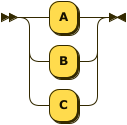
\includegraphics[]{assets/id.png}
          \item [expression: ] 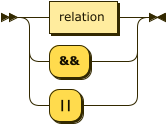
\includegraphics[]{assets/expression.png}
          \item [relation: ] 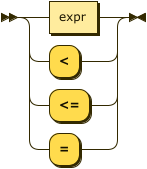
\includegraphics[]{assets/relation.png}
          \item [expr: ] 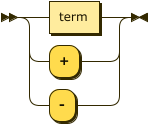
\includegraphics[]{assets/expr.png}
          \item [term: ] 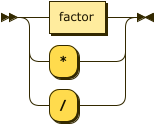
\includegraphics[]{assets/term.png}
          \item [factor: ] 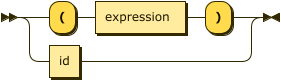
\includegraphics[]{assets/factor.png}
        \end{enumerate}
    \end{enumerate}
  \item For each of the following strings, draw parse trees and abstract syntax trees with respect to the grammar in question 1: 
    \begin{enumerate}
      \item [(a)] (A + B) * C \\
        \begin{enumerate}
          \item [] Parse Tree: \\
            \begin{tikzpicture}
              \node {$\langle expression \rangle$}
                child {node {$\langle relation \rangle$}
                  child {node {$\langle expr \rangle$}
                    child {node {$\langle term \rangle$}
                      child {node {$\langle term \rangle$}
                        child {node {$\langle factor \rangle$}
                          child {node {(}}
                          child {node {$\langle logic \rangle$}
                            child {node {$\langle relation \rangle$}
                              child {node {$\langle expr \rangle$}
                                child {node {$\langle expr \rangle$}
                                  child {node {$\langle term \rangle$}
                                    child {node {$\langle factor \rangle$}
                                      child {node {$\langle id \rangle$}
                                        child {node {A}}
                                      }
                                    }
                                  }
                                }
                                child {node {+}}
                                child {node {$\langle term \rangle$}
                                  child {node {$\langle factor \rangle$}
                                    child {node {$\langle id \rangle$}
                                      child {node {B}}
                                    }
                                  }
                                }
                              }
                            }
                          }
                          child {node {)}}
                        }
                      }
                      child {node {*}}
                      child {node {$\langle factor \rangle$}
                        child {node {$\langle id \rangle$}
                          child {node {C}}
                        }
                      }
                    }
                  }
                };
            \end{tikzpicture}
          \item [] Abstract Syntax Tree: \\
            \begin{tikzpicture}
              \node {*}
                child {node {+}
                  child {node {A}}
                  child {node {B}}
                }
                child {node {C}};
            \end{tikzpicture}
        \end{enumerate} 
      \item [(b)] P \&\& (Q || R + S) \\
        \begin{enumerate}
          \item [] Parse Tree:
            \begin{tikzpicture}
              \node {$\langle expression \rangle$}
                child {node {$\langle relation \rangle$}
                  child {node {$\langle expr \rangle$}
                    child {node {$\langle term \rangle$}
                      child {node {$\langle factor \rangle$}
                        child {node {$\langle id \rangle$}
                          child {node {P}}
                        }
                      }
                    }
                  }
                  child {node {\&\&}}
                  child {node {$\langle relation \rangle$}
                    child {node {$\langle expr \rangle$}
                      child {node {$\langle term \rangle$}
                        child {node {$\langle factor \rangle$}
                          child {node {(}}
                          child {node {$\langle logic \rangle$}
                            child {node {$\langle relation \rangle$}
                              child {node {$\langle expr \rangle$}
                                child {node {$\langle expr \rangle$}
                                  child {node {$\langle term \rangle$}
                                    child {node {$\langle factor \rangle$}
                                      child {node {$\langle id \rangle$}
                                        child {node {Q}}
                                      }
                                    }
                                  }
                                }
                                child {node {||}}
                                child {node {$\langle term \rangle$}
                                  child {node {$\langle factor \rangle$}
                                    child {node {$\langle expr \rangle$}
                                      child {node {$\langle expr \rangle$}
                                        child {node {$\langle term \rangle$}
                                          child {node {$\langle factor \rangle$}
                                            child {node {$\langle id \rangle$}
                                              child {node {R}}
                                            }
                                          }
                                        }
                                      }
                                      child {node {+}}
                                      child {node {$\langle term \rangle$}
                                        child {node {$\langle factor \rangle$}
                                          child {node {$\langle id \rangle$}
                                            child {node {S}}
                                          }
                                        }
                                      }
                                    }
                                  }
                                }
                              }
                            }
                          }
                          child {node {)}}
                        }
                      }
                    }
                  }
                };
            \end{tikzpicture}
          \item [] Abstract Syntax Tree: \\
            \begin{tikzpicture}
              \node {\&\&}
                child {node {P}}
                child {node {||}
                  child {node {Q}}
                  child {node {+}
                    child {node {R}}
                    child {node {S}}
                  }
                };
            \end{tikzpicture}
        \end{enumerate}
    \end{enumerate}
  \item Prove that grammar is ambiguous \\
    \begin{tikzpicture}
      \node {$\langle S \rangle$}
        child { node {$\langle A \rangle$}
          child { node {$\langle A \rangle$}
            child { node {$\langle A \rangle$}
              child { node {$\langle id \rangle$}
                child { node {a} }
              }
            }
            child {node {-}}
            child {node {$\langle A \rangle$}
              child {node {$\langle id \rangle$}
                child {node {b}}
              }
            }
          }
          child {node {+} }
          child {node {$\langle A \rangle$}
            child {node {$\langle id \rangle$}
              child {node {c} }
            }
          }
        };
    \end{tikzpicture}
    \begin{tikzpicture}
      \node {$\langle S \rangle$}
        child { node {$\langle A \rangle$}
          child { node {$\langle id \rangle$}
            child { node {a} }
          }
          child {node {-} }
          child {node {$\langle A \rangle$}
            child { node {$\langle A \rangle$}
              child { node {$\langle id \rangle$}
                child { node {b} }
              }
              child {node {+}}
              child {node {$\langle id \rangle$}
                child {node {c}}
              }
            }
          }
        };
    \end{tikzpicture}
  \item Write a regular expression for floating-point numbers \\
    % [+ | -] ? [[0]? | [1-9]+].[\d]+
    \verb/^[\+|\-]?0?\.\d+$|^[\+|\-]?[1-9]+\d+\.\d+$/
    % $\^[\backslash+ |\; \backslash-]?[0?\; |\; [1 - 9]+ \backslash d+ ]\backslash.\backslash d+\$$
    % \[\\\+ | \\\-\]?\[0? | \[1-9\]\+\]\'.\'\[\\d\]\+
\end{enumerate}

\end{document}